\newpage
\section{Results and Analysis}
\label{chapter:analysis}

% SECTIONS
% Results

% Analysis
% What the hell is going on? Why are the strongest results in violation of the order? (Is the order interpreted in the wrong direction?...)

% Ablation study, Sensibility analysis of hyperparameters
% Weaknesses (in relation to assumptions)

% Selecting only compliant relations: there's just very few left, they happen to be wrong?

\subsection{Receiver Operating Characteristic Curves}

We first analyse the performance of order-based LCD on the \citet{kemmeren2014large} dataset using the receiver operating characteristic (ROC) curve. This graph shows the number of true positives versus false positives of a binary classifier as a prediction threshold is varied. Good methods rise quickly and make many good predictions before starting to make mistakes. Specifically, we fix a binary ground-truth that defines the true ancestral relations between genes. The aggregated scores resulting from the bootstrapped experiment are thresholded to select predictions that are tested to the ground-truth.

\subsubsection{Compared to Other Methods}

In the top row of Figure \ref{fig:7:rocgen} we show the ROC curves of order-based LCD, ICP which is considered the best method on this data, the L$_2$-boosting baseline and a random baseline. We computed the curves for the $10\%$, $1\%$, and $0.1\%$ strongest relations according to the absolute score. The discrete predictions of the methods are used. The ROCs of other combinations of these settings, including standardized scores and continuous predictions, can be found in Appendix \ref{appendix:roc}. The conclusions hold for all settings.

\begin{figure}[h]
    \centering
    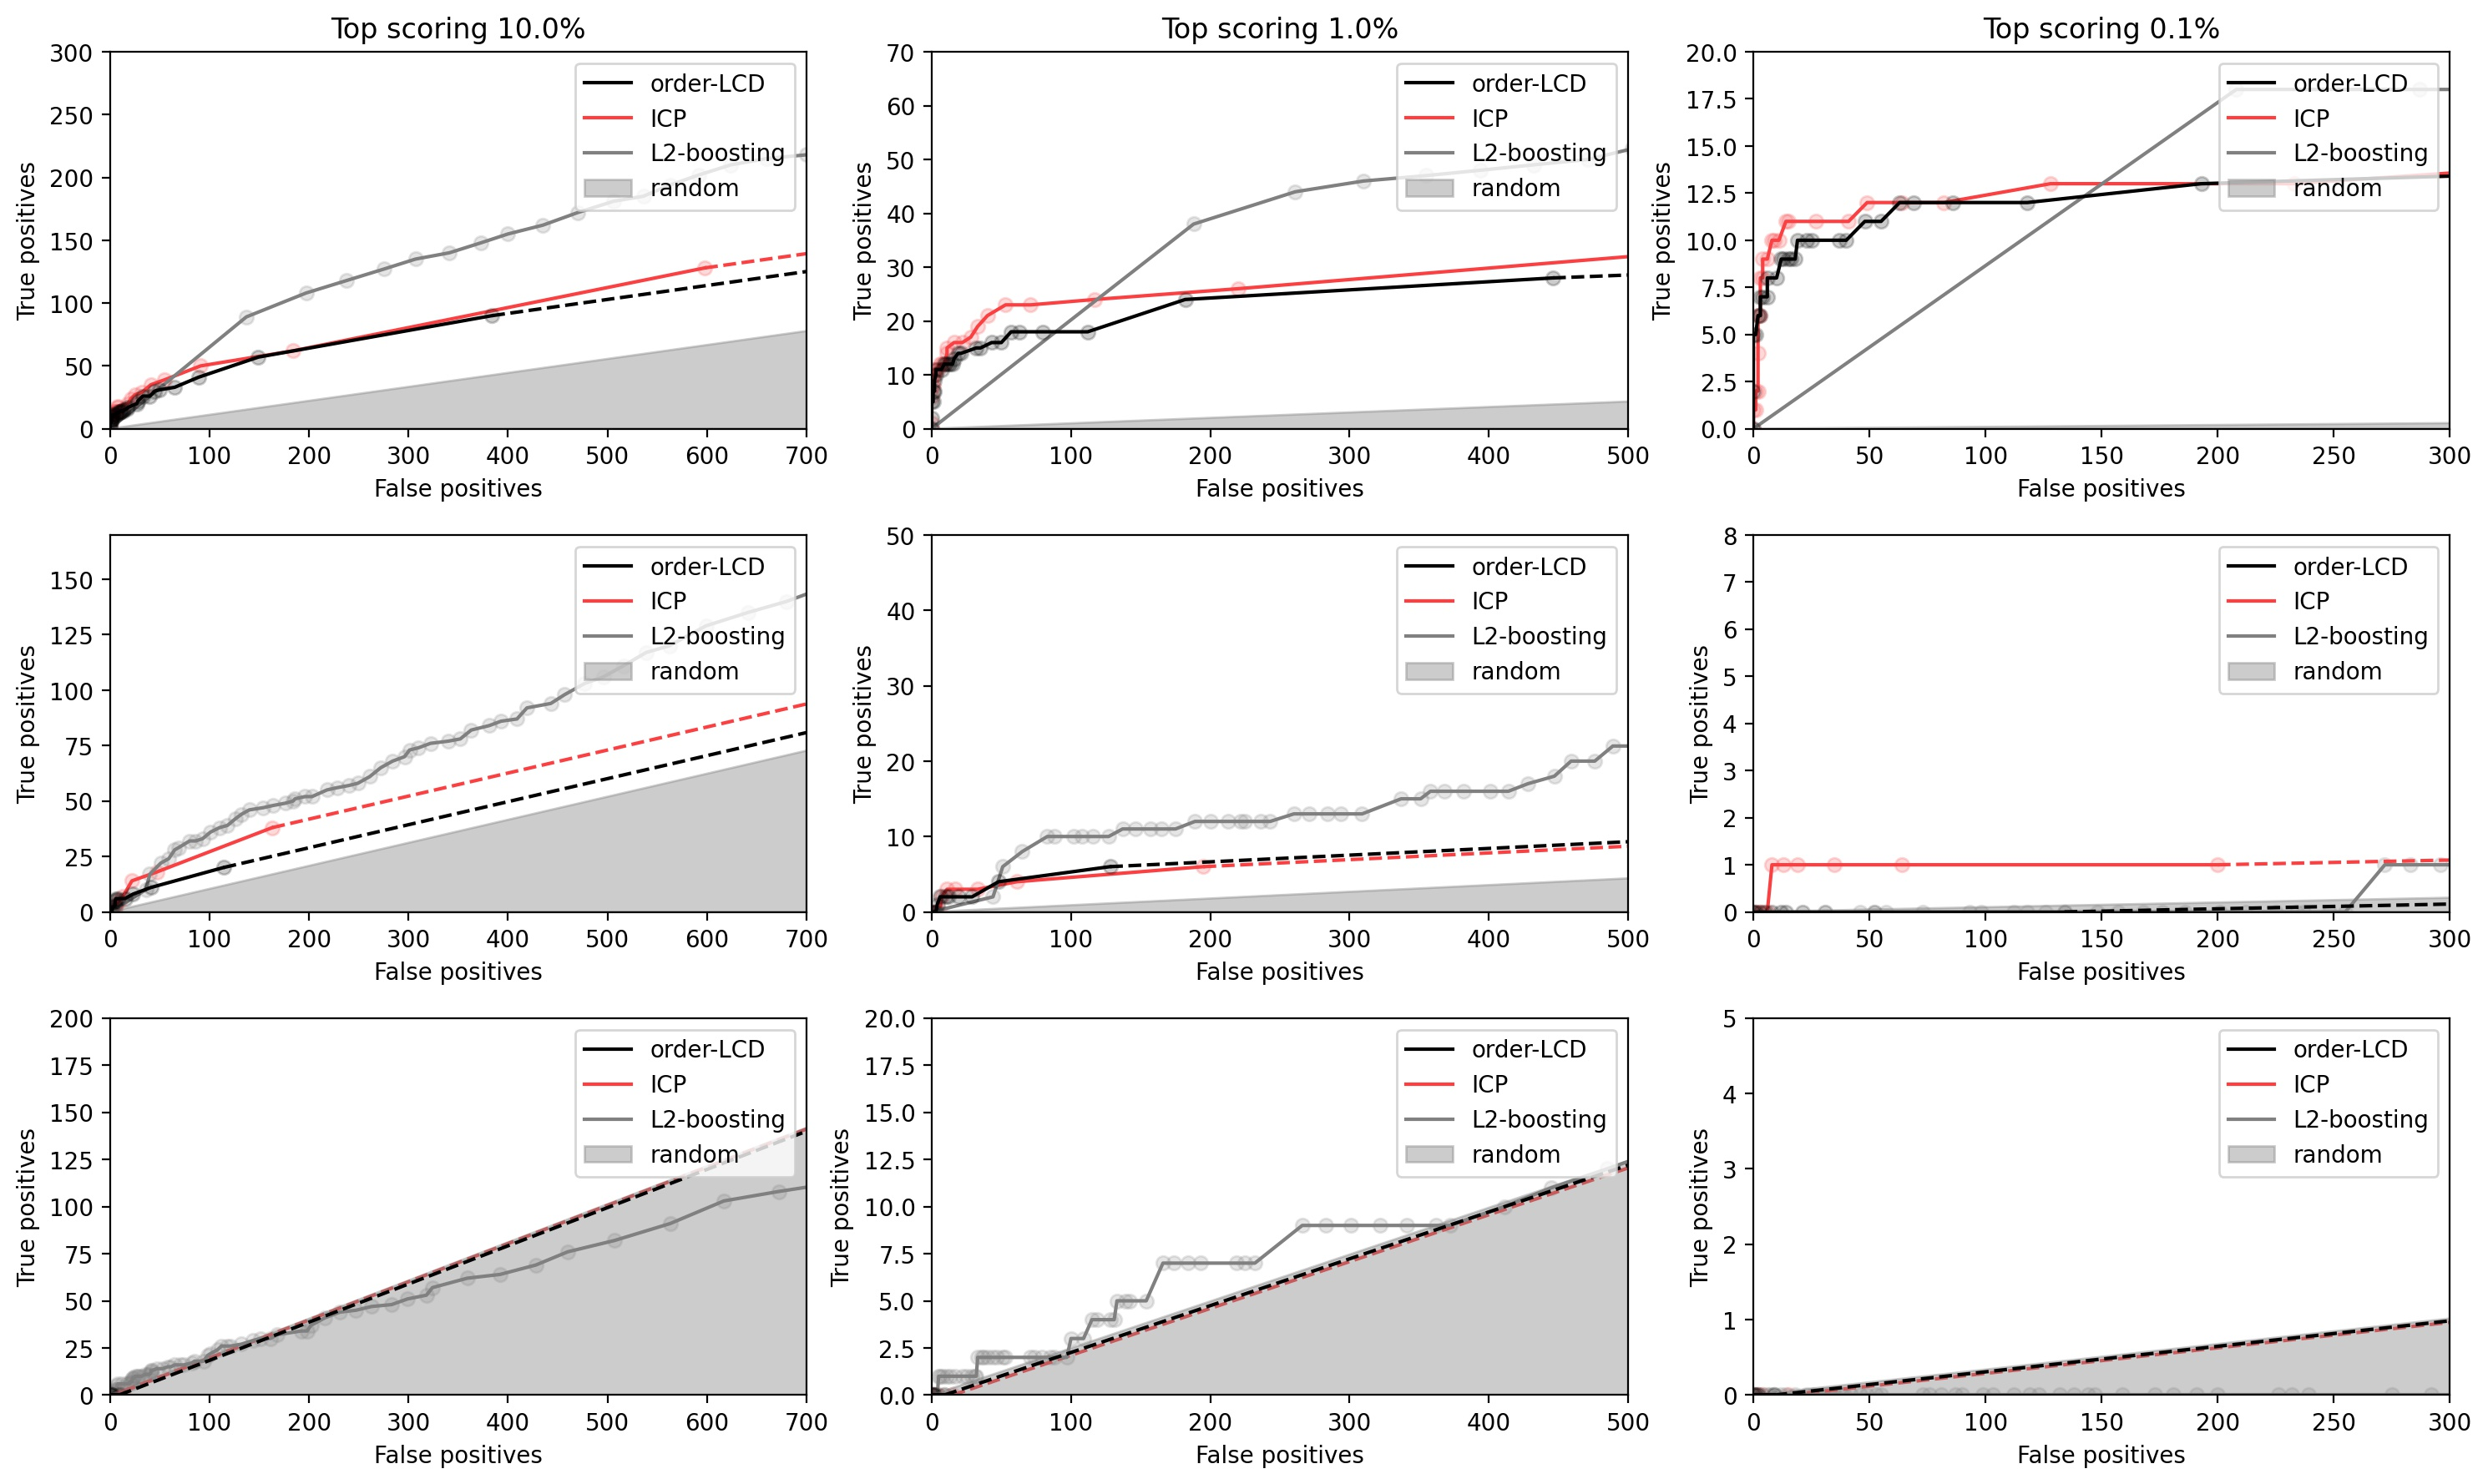
\includegraphics[width=\textwidth]{7roc_general.jpg}
    \caption{ROC curves of order-based LCD compared to other methods. Columns use different ground-truth thresholds, rows different subsets of the relations that are evaluated. A dashed line indicates that a method resorts to random guessing.}
    \label{fig:7:rocgen}
\end{figure}

Order-LCD and ICP beat the L$_2$-boosting baseline in their most confident predictions. The first 10 predictions are generally very good. After this point the methods quickly start making many mistakes. This indicates the hardness of this prediction task.

Most importantly, we see that order-based LCD approaches the performance of ICP. This is a desirable result, because order-based LCD is a more efficient method than ICP and may therefore be used as a fast approximation. Note that this conclusion was initially drawn about LCD by \citet{versteeg2019boosting}, which inspired the adaptation of the method in this thesis. A comparison to this LCD method follows in the next subsection.

Besides these ROC curves, two more settings were tested in which only a subset of ancestral relations is considered. These graphs can be found in the second and third row of Figure \ref{fig:7:rocgen}. The \textit{intervention table} ROC curve is only concerned with relations between genes that occur as knock-out in the data. These predictions may be considered as a different task, as this subset of genes may be qualitatively different from the rest since it was chosen by \citet{kemmeren2014large} based on some biological criteria. 

We may expect that order-based LCD behaves differently on this subset of ancestral relations. The inferred order is purely based on this intervention table, and the order inference algorithm is chosen based on analysis of this table. However, the results are not qualitatively different. Only the first few predictions of order-based LCD and ICP beat the L$_2$-boosting baseline.

The \textit{order-compliant relations} ROC curve contains only those relations that are explicitly not in violation of the order inferred by order-LCD. This small subset of ancestral relations may be used to test whether order-LCD performs relatively well on those relations that are most in line with our hypothesis. Do the genes comply to some implicit order, and can this be used to inform the context variable of LCD? Unfortunately, very little predictions in this subset are made by order-based LCD or ICP. It may be that this small subset of relations happen to be harder to prove, or that order-based LCD fails to show the relations that it was designed for. The fact that the L$_2$-boosting baseline performs about as good, or worse than the random baseline on this subset supports the first explanation.


\subsubsection{Compared to LCD Methods}

Figure \ref{fig:7:roclcd} shows ROC curves of all methods related to LCD. The most important result is that the ROC curves of the original LCD and our order-based LCD are very similar. This means that we failed in our attempt to improve on the original LCD by informing the context with some gene ordering. We analyse the small difference between these two methods in the end of this section.

Figure \ref{fig:7:roclcd} also shows the results of an ablation study. We randomized the inferred order, the inferred gene positions, and both together, to investigate to what extend these additions to the original LCD contribute to the performance of order-based LCD. Although order-based LCD is not beaten by its randomized versions in the strongest predictions, the difference is never more than a few true positives. We have to conclude that we failed to show a significant effect of our order inference and our position inference. This may show that the approach is not effective on this dataset, or that order inference or position inference should be implemented differently to benefit LCD. Since position inference was not as extensively developed in this thesis, the problem may lie there.

\begin{figure}[h]
    \centering
    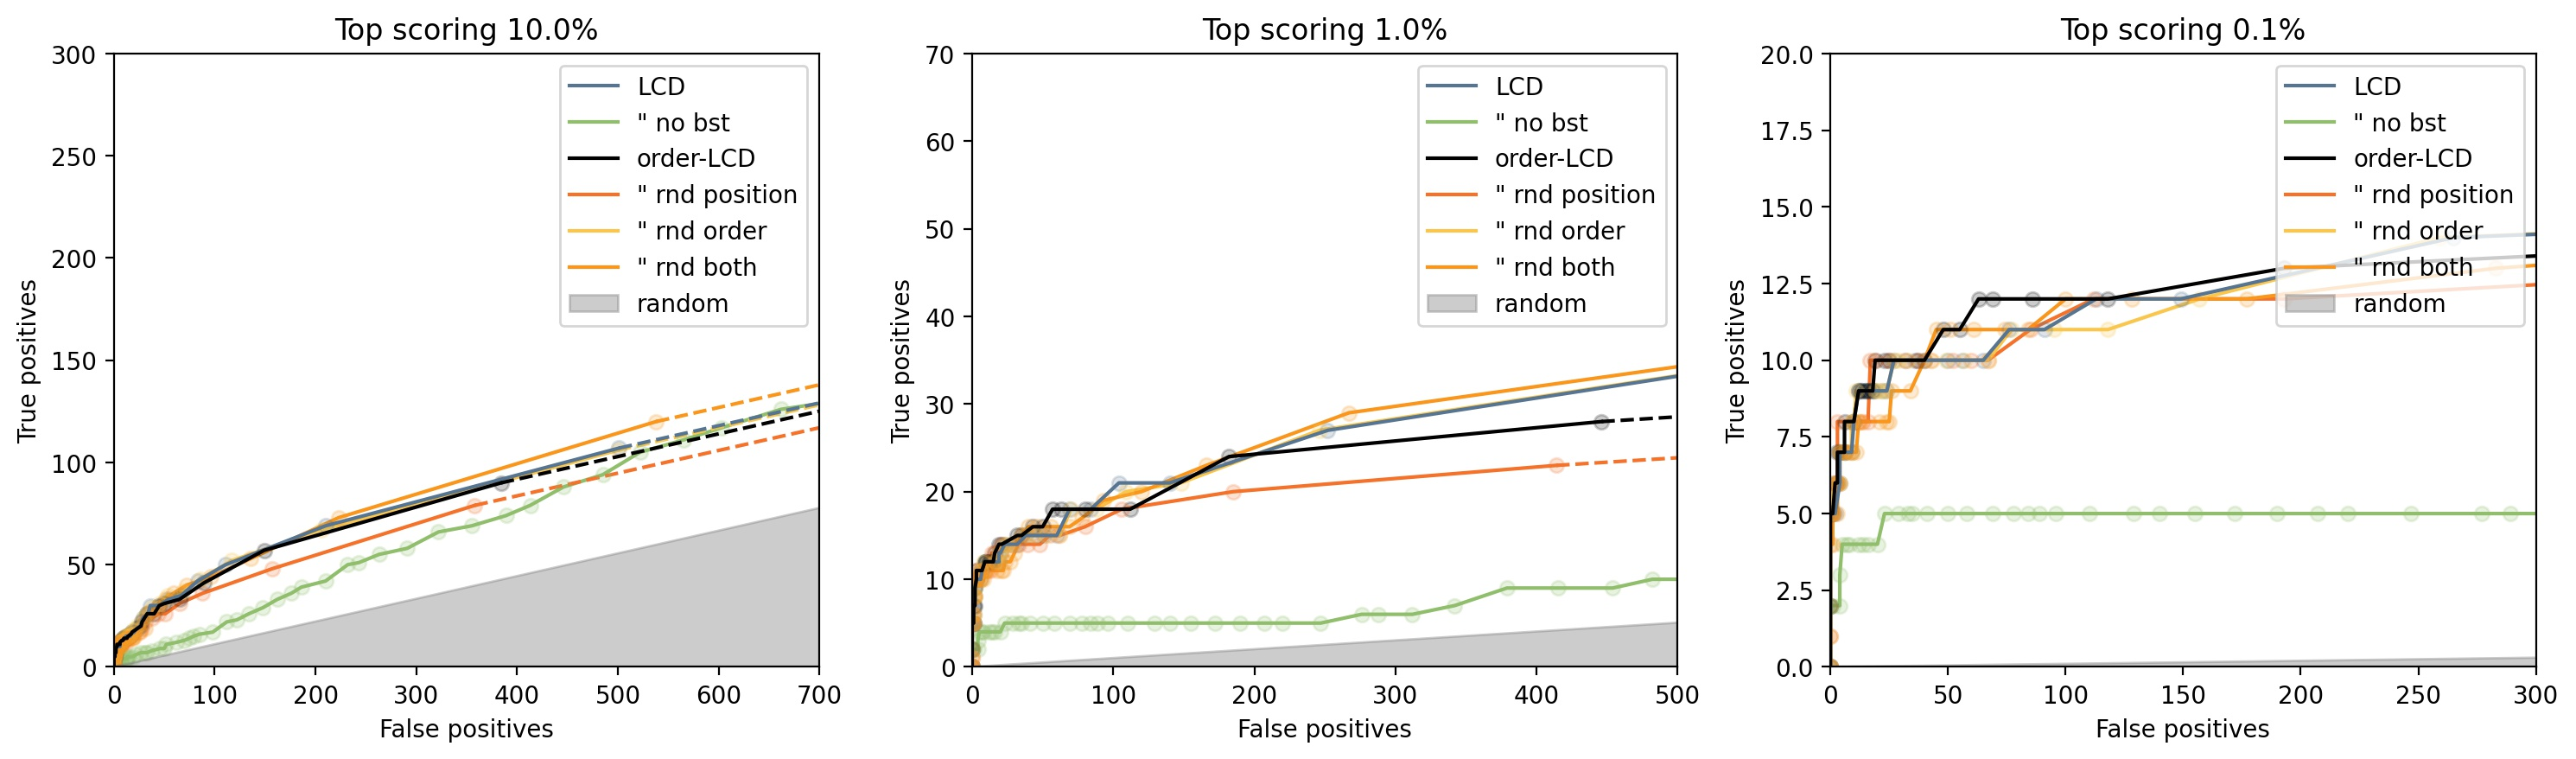
\includegraphics[width=\textwidth]{7roc_lcd.jpg}
    \caption{ROC curves of order-based LCD compared to other LCD methods. Columns use different ground-truth thresholds. A dashed line indicates that a method resorts to random guessing.}
    \label{fig:7:roclcd}
\end{figure}

\subsection{Accumulated Regression Deviation}

We provide another approach to evaluate the performance of the algorithms to show that our conclusions extend beyond binary ground-truths and ROC curves. When some method predicts an ancestral relation, we use the data in the train split to predict a precise expression value of the knock-out. Figure \ref{fig:7:contex} shows how this is computed. Using the joint data or only the intervention data, we apply linear regression and use it to predict a deviation at the knock-out value of the cause gene. Note that we are cheating a little here, since this knock-out value is not in the train split. If the results of this approach were great, we could redefine the metric to see if the results are robust. For example, we could assume a standard knock-out value of about $-2.5$.

\begin{figure}[h]
    \centering
    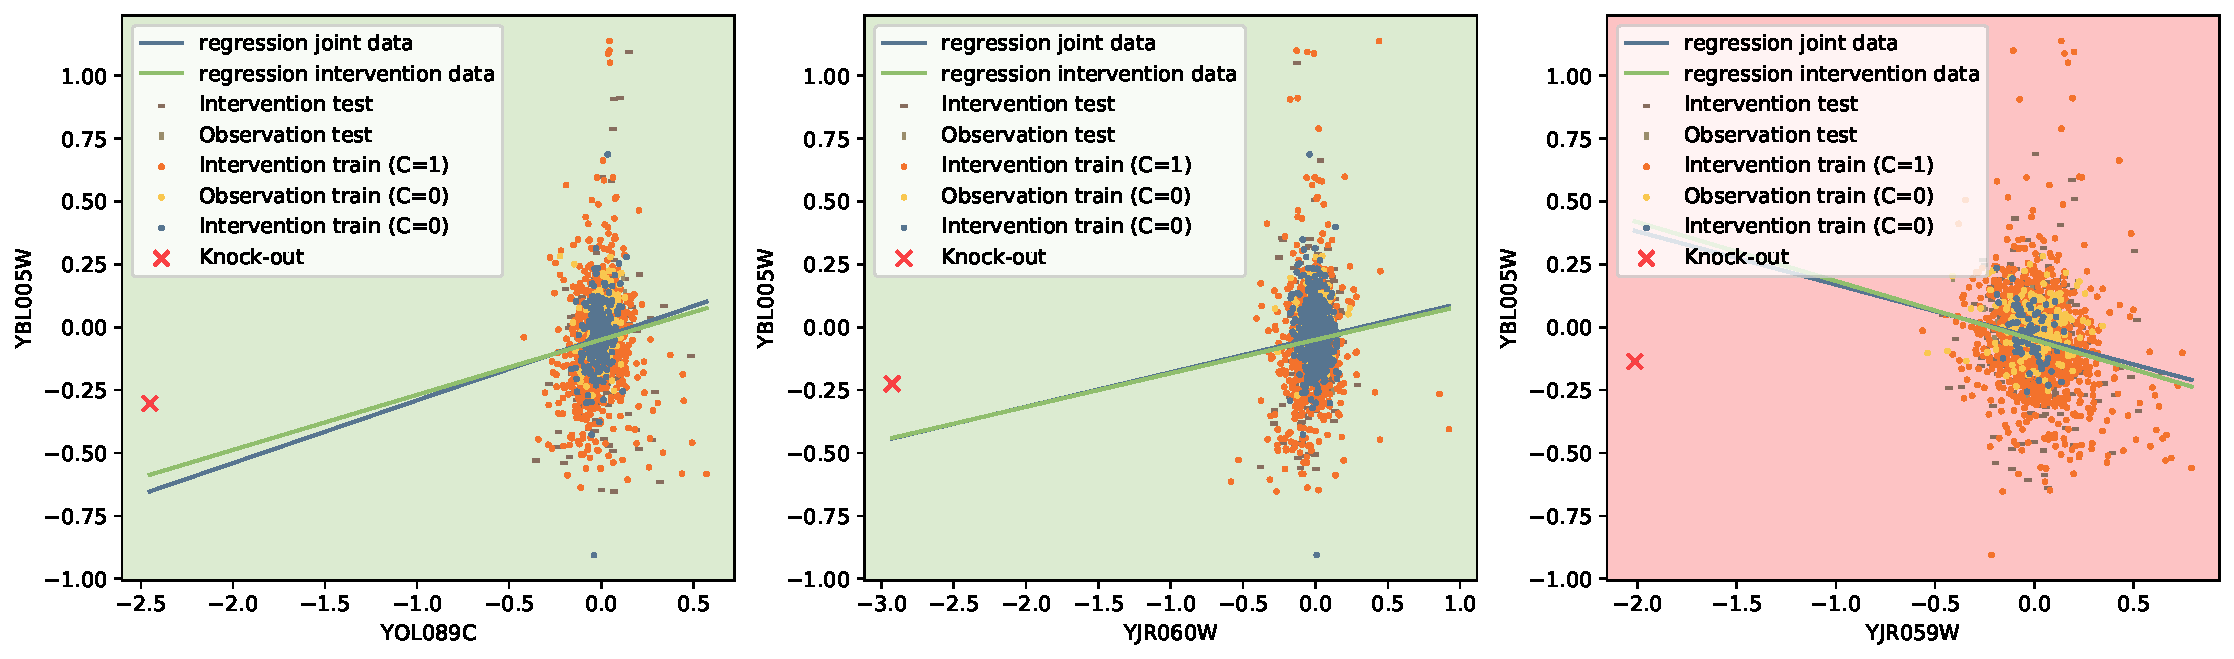
\includegraphics[width=\textwidth]{7contin_example.pdf}
    \caption{Visualization of regression deviation. Linear regression is applied to the joint or intervention train data. The deviation is the vertical distance between the regression line and the red knock-out cross.}
    \label{fig:7:contex}
\end{figure}

\begin{figure}[p]
    \centering
    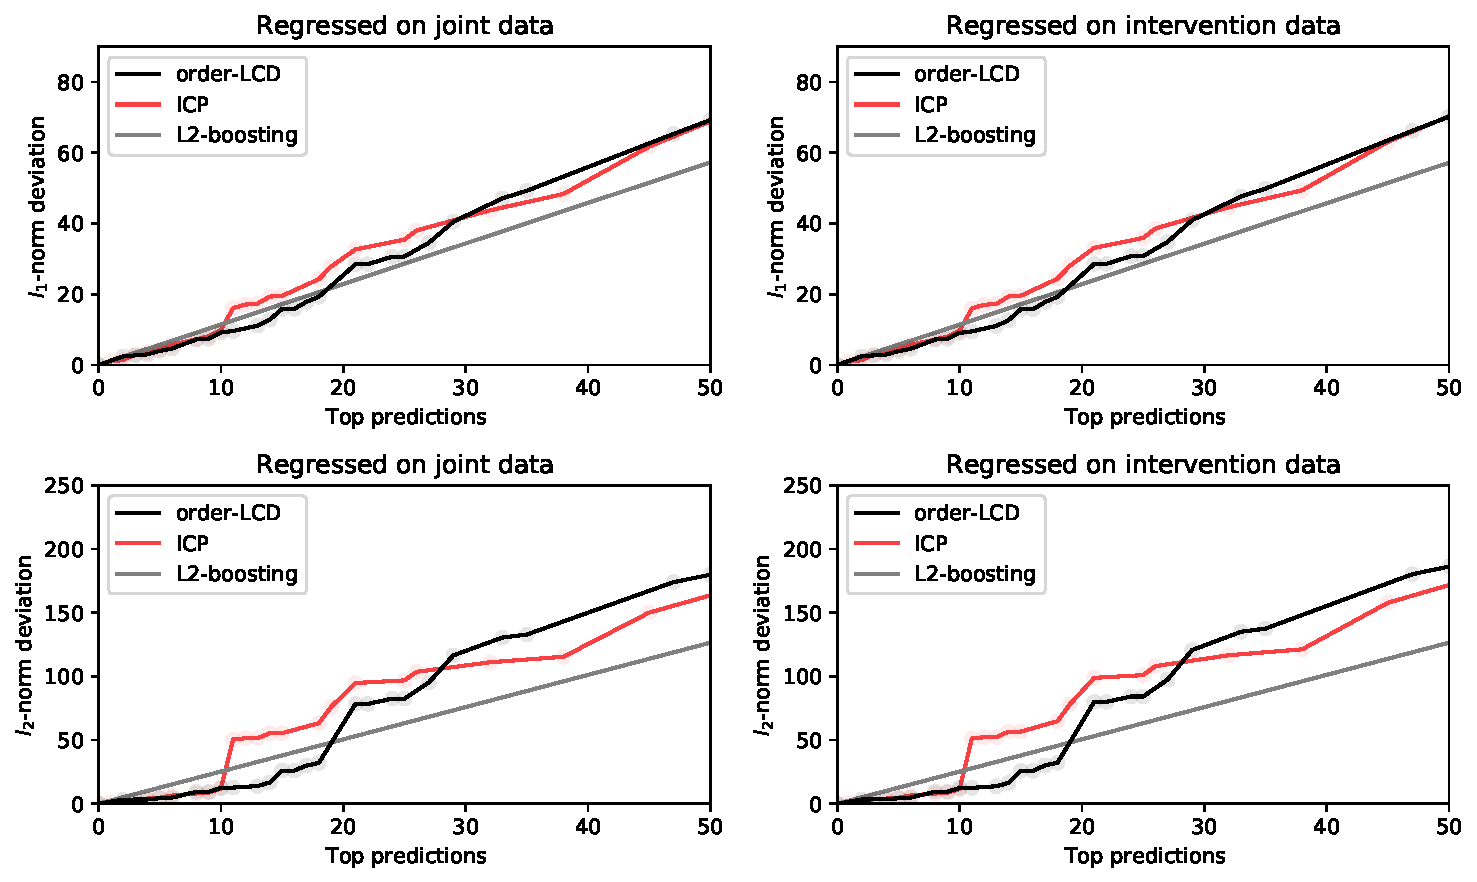
\includegraphics[width=\textwidth]{7contin_general.pdf}
    \caption{Accumulated regression deviation of order-based LCD compared to other methods. Columns use different data to regress on, rows a different norm to add the accumulated deviations.}
    \label{fig:7:congen}
\end{figure}

\begin{figure}[p]
    \centering
    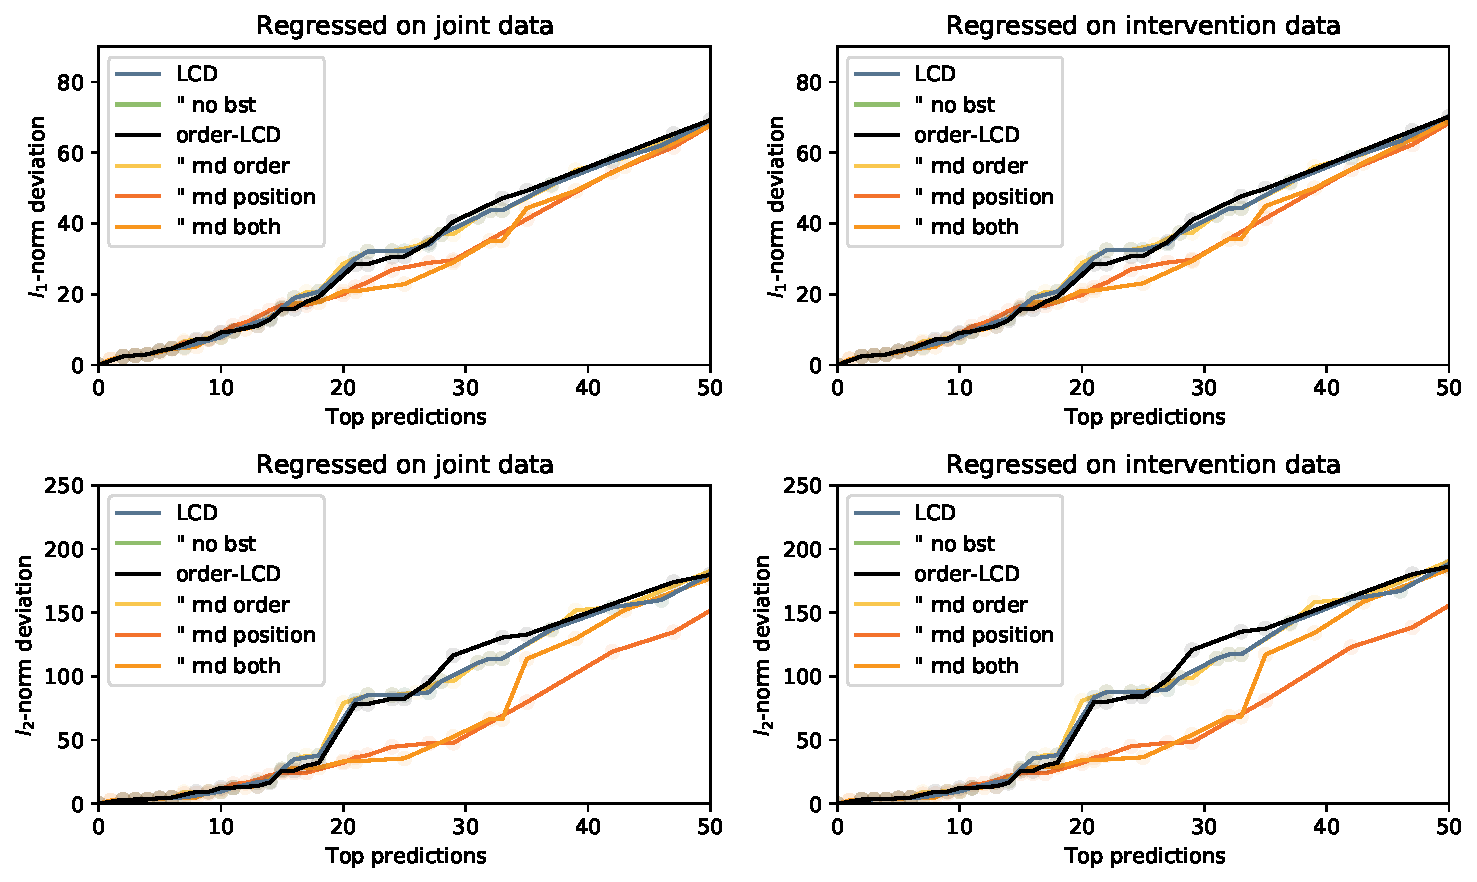
\includegraphics[width=\textwidth]{7contin_lcd.pdf}
    \caption{Accumulated regression deviation of order-based LCD compared to other LCD methods. Columns use different data to regress on, rows a different norm to add the accumulated deviations.}
    \label{fig:7:conlcd}
\end{figure}

To compare the performance of the most confident predictions of different algorithms, we create accumulated regression deviation graphs. These accumulate the deviations of the top predictions using the $l_1$-norm or $l_2$-norm.\footnote{The $l_1$-norm is the sum of absolute values, the $l_2$-norm is the sum of squared values.} Better methods have graphs with low accumulated deviation for the top predictions.

Figure \ref{fig:7:congen} shows the graphs for order-based LCD compared to ICP and the L$_2$-boosting baseline. Again, both methods beat the baseline for the strongest predictions in all settings. Interestingly, order-based LCD seems to take longer to degrade than ICP. This result was not further investigated in this thesis.

The graphs comparing the LCD methods is shown in Figure \ref{fig:7:conlcd}. In the top 20 predictions we see hardly any difference, besides that boosting improves performance. Generally, we again struggle to see a significant difference between the original LCD and order-based LCD. 

A surprising result shows up when we consider the ablation experiments. Further in the graph, it seems that randomizing the inferred positions leads to a better performance. Note that we decided to make position inference relatively strict, by putting many genes near the end of the order. The randomized position version indicates that we may expect better performance on this metric if we infer the positions more spread out. 

A last remark is that linear regression is related to the independence tests that are used by the algorithms. In the accumulated deviation graphs we observe that there is hardly a difference between regression on joint data and intervention data. This shows that adding observation data changes very little about the regression. A new task could be defined in which a subset of the intervention data is selected for regression. Using the same intuition from this thesis, we may hypothesize that selecting the interventions on ancestors yields a better prediction of knock-out expression.

% Generalize to continuous score settings?


\subsection{Comparison of Order-Based LCD with Original LCD}

\subsubsection{Specific examples}


\begin{figure}[p]
    \centering
    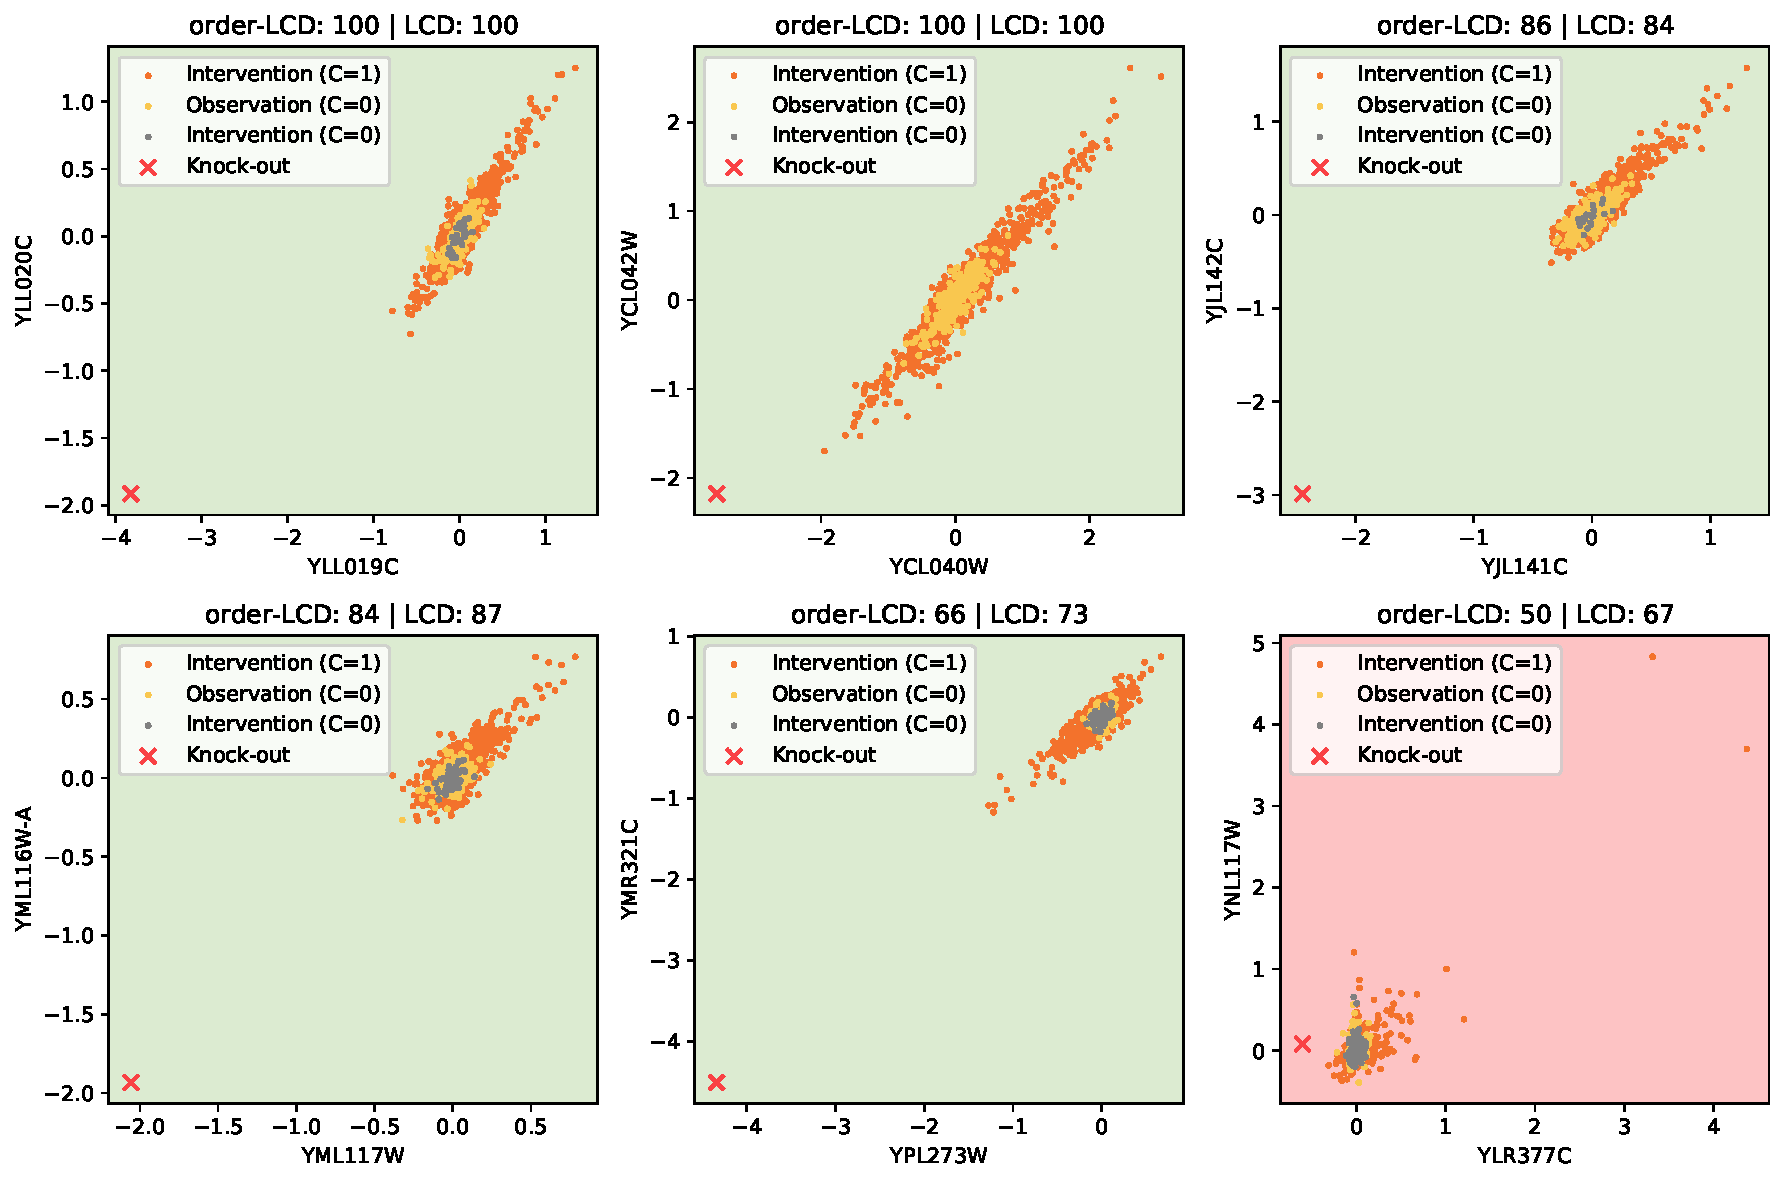
\includegraphics[width=\textwidth]{7inclusive.pdf}
    \caption{The six strongest predictions by order-based LCD that are also predicted by LCD. The precise scores are shown above the figures. The background color indicates whether the relation is true according to the $10\%$ threshold.}
    \label{fig:7:exincl}
\end{figure}

\begin{figure}[p]
    \centering
    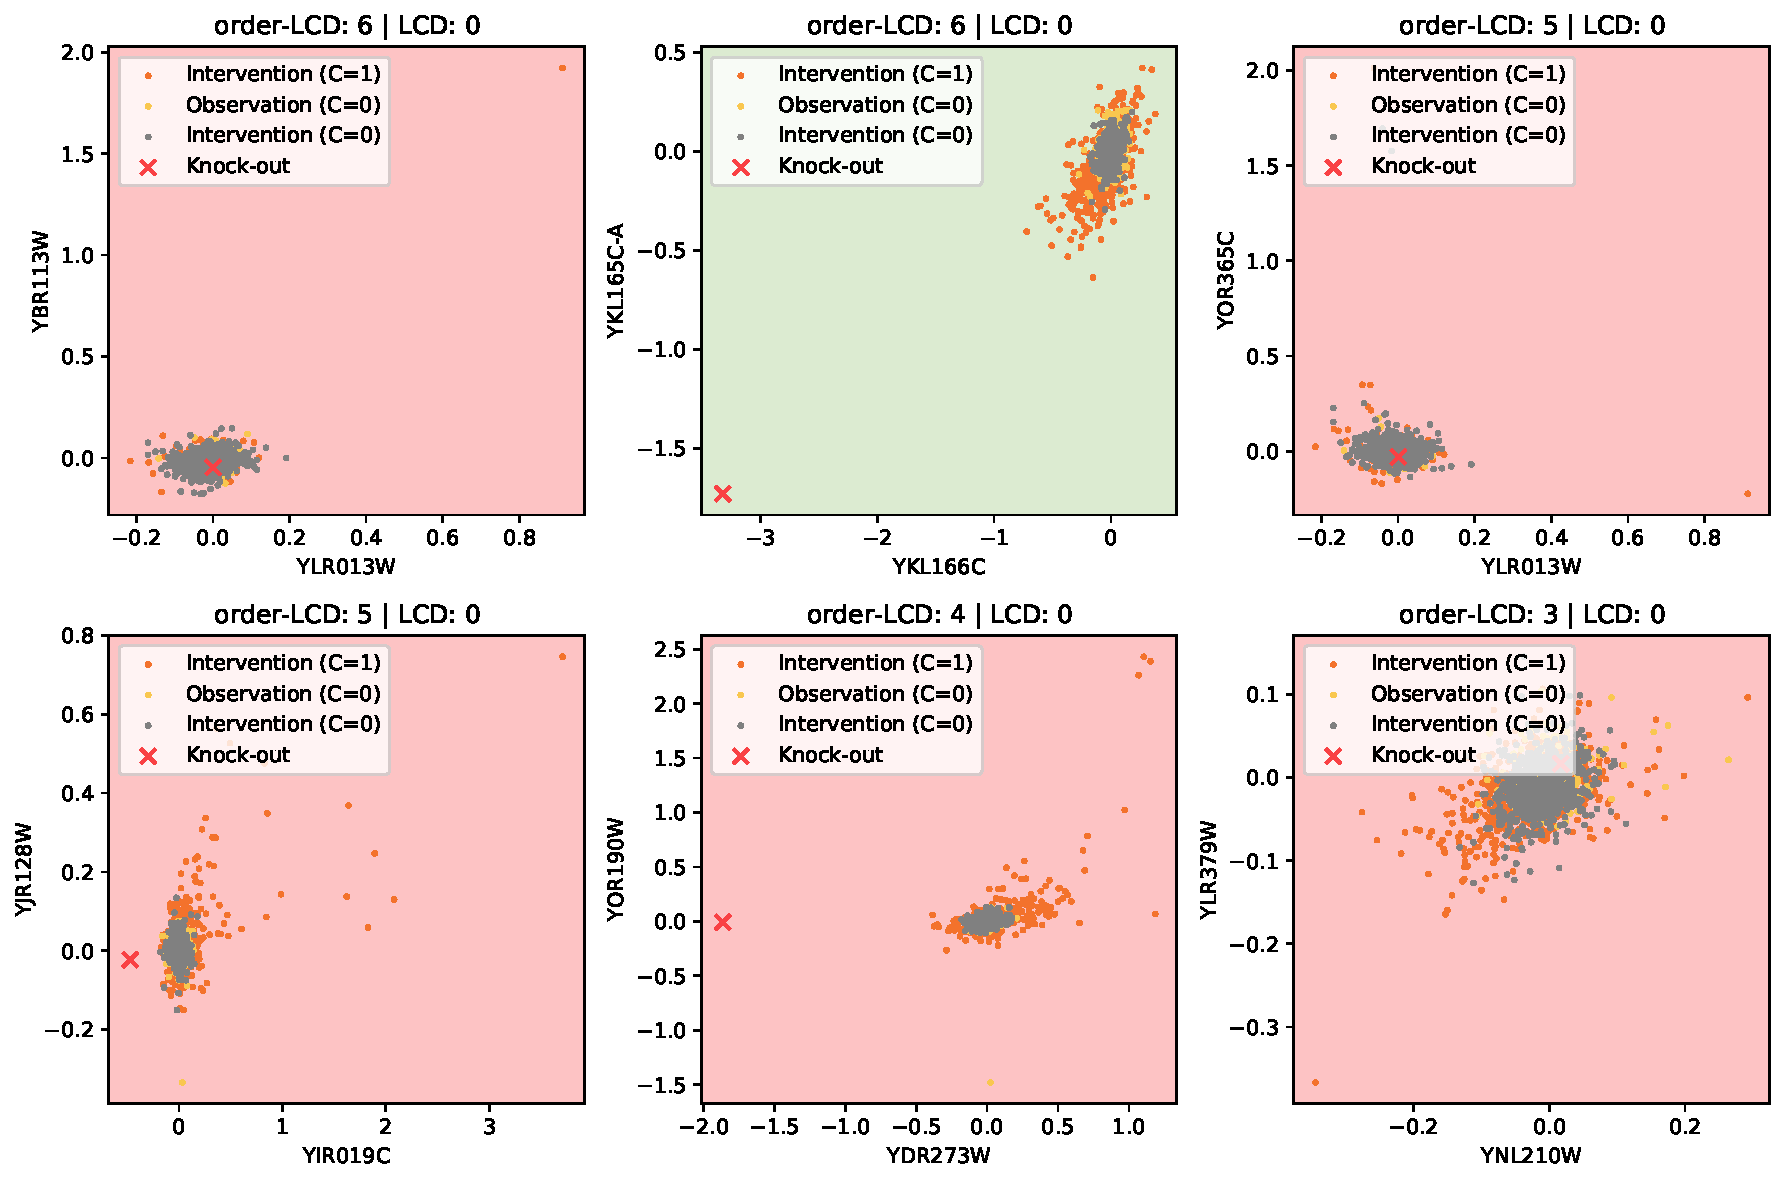
\includegraphics[width=\textwidth]{7exclusive.pdf}
    \caption{The six strongest predictions by order-based LCD that are not predicted by LCD. The precise scores are shown above the figures. The background color indicates whether the relation is true according to the $10\%$ threshold.}
    \label{fig:7:exexcl}
\end{figure}

We investigate qualitatively how the predictions of order-based LCD are related to those of the original LCD. Figure \ref{fig:7:exincl} shows the six strongest predictions of order-based LCD that are also predicted by LCD, the top 25 can be found in Appendix \ref{appendix:roc}. It can be observed that these relations are also strongly predicted by LCD, and most are correct. The only relation that is wrongly predicted by both methods obtains a higher score from the original LCD, which gives some hope for the order-based method. All relations have relatively little intervention data that obtains context value $0$, which means that both methods are very similar. In one case, none of the interventions obtain this context value and the methods are effectively identical. 

More interesting are the strongest order-based LCD predictions that are not at all predicted by LCD. The top six is shown in Figure \ref{fig:7:exexcl}, and the top 25 in Appendix \ref{appendix:roc}. We would hope that the methods behave differently, and that order-based LCD improves over LCD by making some entirely new, confident predictions. This is not what we see. The strongest exclusive prediction has merely a score of $6/100$. Interestingly, these relations assign many intervention points the context value $0$, and are in that way able to make predictions where the original LCD cannot. Unfortunately, most of these exclusive relations are also wrong, even according to the weak $10\%$ binary ground-truth. 


\subsubsection{General Similarity}

Finally, we take a more general approach in the comparison of order-based LCD and the original LCD, and try to explain why we failed to show a clear difference between the methods. 

Figure \ref{fig:7:excltotals} shows that the distribution of prediction scores assigned by order-based LCD and the original LCD are very similar. Furthermore, only low scores are assigned to exclusive relations, that are predicted by one method but not by the other. 

\begin{figure}[h]
    \centering
    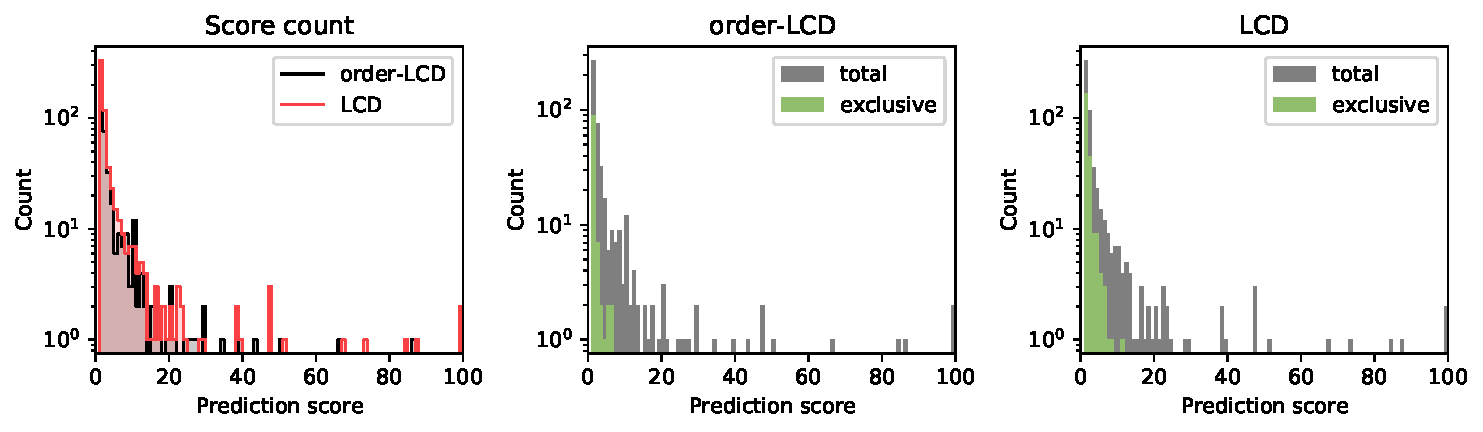
\includegraphics[width=\textwidth]{7exclusive_totals.pdf}
    \caption{Comparing the distribution of discrete prediction scores of order-based LCD and the original LCD. Left: distribution of scores of both methods. Middle: distribution of order-based LCD, and distribution of the scores assigned to relations not predicted by LCD. Right: same, but comparing LCD to order-based LCD.}
    \label{fig:7:excltotals}
\end{figure}

Figure \ref{fig:7:scorevs} further shows that when we sort predictions from strong to weak, both methods end up with a very similar order. The strongest relations of order-based LCD are also the strongest ones of LCD. Weak relations of order-based LCD are also weak according to LCD. 

\begin{figure}[h]
    \centering
    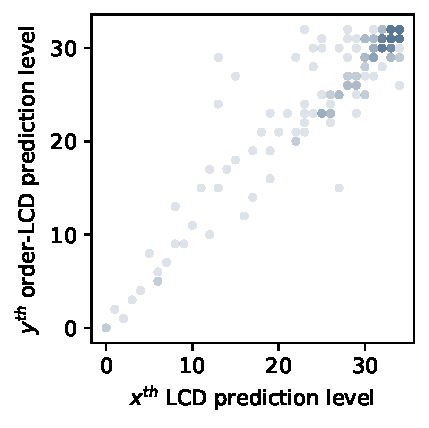
\includegraphics[width=.3\textwidth]{7score_vs.pdf}
    \caption{Comparing how predictions of order-based LCD and the original LCD are related, going from strongest to weakest predictions. A prediction level contains relations that are assigned the same score, and can therefore not be ordered among themselves.}
    \label{fig:7:scorevs}
\end{figure}

Since we showed in many ways that both methods are very similar. We expect that this is the case because the position inference algorithm is chosen to be too conservative. In Chapter \ref{chapter:methodcontext} we chose a middle way between the desirable properties of a very spread out distribution of inferred gene positions, and inferred positions that hardly precede the actual position according to the order inference algorithm. The chosen middle way still resulted in most positions to be pushed to the end of the order, therefore keeping most of the context values $1$. Note that pushing a position all the way to the back means that all context is one, rendering the method identical to the original LCD. Simply put, if we spread out the positions more, then the method becomes more different from the original LCD. 

Figure \ref{fig:7:contexthist} shows the distribution of the cause variable expressions in the data, for the five causes in the strongest predictions of order-based LCD. The expressions are separated in three clusters, corresponding to the data source (observation or intervention) and the assigned context value. Ideally, in the cluster with context value $1$, we collect those interventions that are affected by the cause variable. In this thesis we attempt to estimate this with an order in the genes. In the figure, we would then like to see that the extremes of the intervention data are assigned $C=1$, whereas many values in the center are assigned $C=0$. This would correspond to interventions that clearly affect the cause variable being assigned to the $C=1$ cluster. 

\begin{figure}[h]
    \centering
    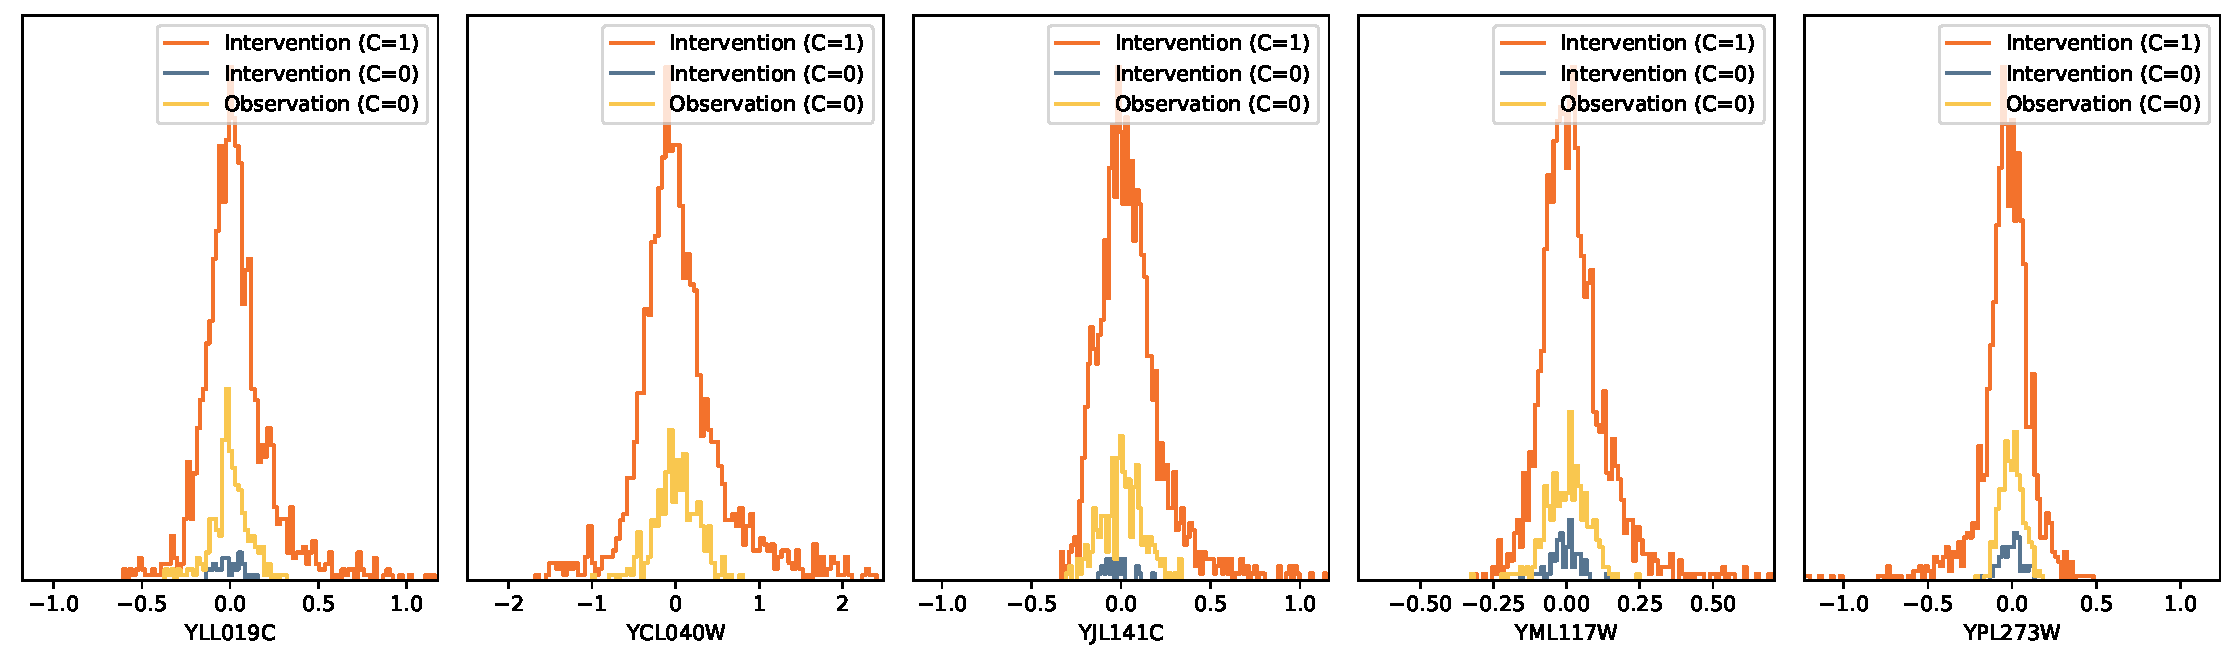
\includegraphics[width=\textwidth]{7context_hist.pdf}
    \caption{Distribution of the expression level of the cause genes in the strongest predictions of order-LCD. Clusters are made based on whether the data points are observation or intervention data, and based on the context value if the data point is interventional.}
    \label{fig:7:contexthist}
\end{figure}

In Figure \ref{fig:7:contexthist} we fortunately see that no data points in the extremes are assigned to $C=0$. However, also very little central data points are assigned to $C=0$. This means that the difference in the data used by the independence tests of order-based LCD and the original LCD are very similar, and we would indeed not expect large differences. 








% \subsubsection{Old stuff}

% % ROCs
% We evaluate the methods using receiver operating characteristic (ROC) curves. The methods assign a score to every causal relation. The ROC curves plot how the number of true positives and false positives change for different thresholds on this score. Each method only assigns a score to some relations. If we require predictions beyond this point, we can only guess randomly.

% The ROC curves in Figure \ref{fig:7:rocshort} are discussed in detail in this section. For each method, we aggregated continuous predictions and evaluated on the absolute score ground-truth. The curves for other settings are shown in Appendix \ref{appendix:roc}. The conclusions that we draw here are applicable to the other settings as well.

% ROC curves show the number of true positives on the x-axis versus false positives on the y-axis. Good methods rise quickly. Figure \ref{fig:7:rocshort} shows different ways to evaluate the same methods. Each column represents a different ground-truth threshold. This threshold indicates the percentage of top scoring relations that are considered to be true. Each row represents an evaluation filter. Methods are evaluated on the full dataset, the intervention table, and the relations that are explicitly compliant to the inferred order and test variable position. After the last prediction of a method, we indicate random guessing with a dashed line.

% We first recapitulate the main findings of \citet{versteeg2019boosting} about the baseline methods. Then we compare order-based LCD to them. Finally we discuss the effect of preselection to our method.

% % \begin{figure}[h]
% %     \centering
% %     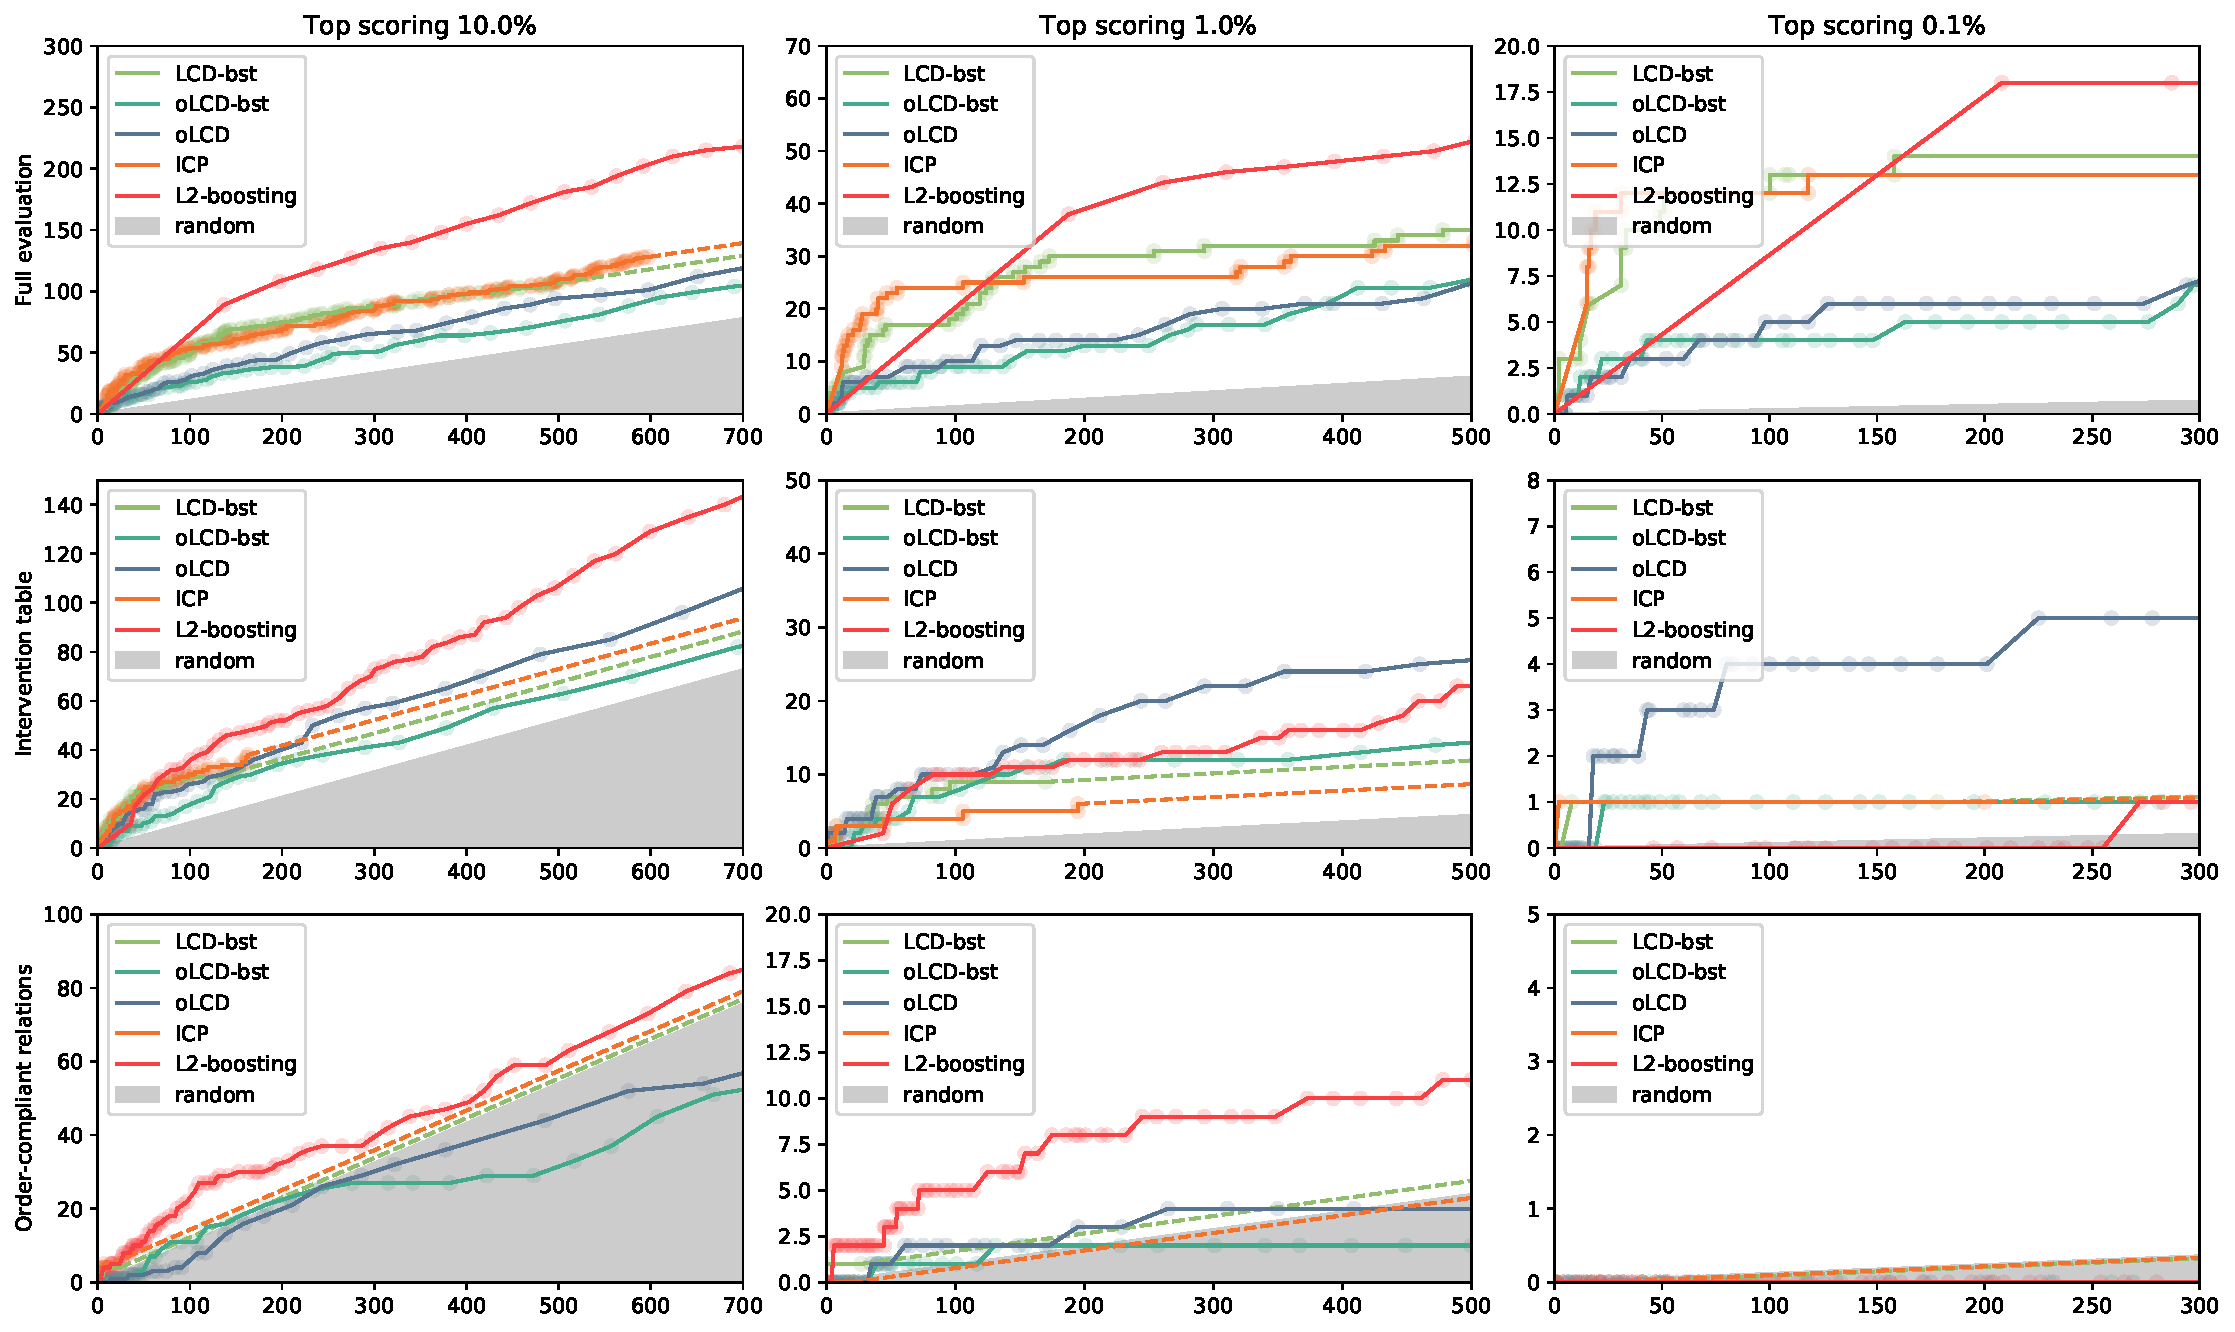
\includegraphics[width=\textwidth]{ROC_filter_threshold_absgt_scorespred_short.pdf}
% %     \caption{Partial ROC curve using the absolute ground-truth with aggregation of continuous scores.}
% %     \label{fig:7:rocshort}
% % \end{figure}

% \subsubsection{Baselines}

% % ICP/LCD is more fine-grained at start
% Since we compare order-based LCD to the baseline methods of \citet{versteeg2019boosting}, we first summarize their findings\footnote{The exact ROC curves of that paper can be found in Appendix \ref{appendix:roc}, in the top row of Figure \ref{fig:app:rocversteeg}}. 226 relations are predicted in all subsamples by the non-causal L$_2$-boosting baseline. They are shown as the first point in the ROC curves. When we wish to use this method to make fewer predictions, we can only guess randomly within this set. The predictions of ICP and LCD are more fine-grained, because their 200 strongest predictions contain multiple confidence levels. LCD and ICP have many more true positives in their top 70 than L$_2$-boosting, as can be seen in the top row of Figure \ref{fig:7:rocshort}. This is where the non-causal baseline is beaten.

% % LCD is largely explained by L2
% Moreover, \citet{versteeg2019boosting} investigate the impact of L$_2$-boosting preselection on LCD. Preselection improves the method significantly. Preselection is what makes LCD comparable to ICP, being computationally less expensive. LCD can be interpreted as a causal filter on the non-causal L$_2$-boosting baseline. The baseline works surprisingly well on its own. The LCD conditions are a causal check that filter out mistakes of in the baseline, specifically causation in the opposite direction and confounding.

% % LCD does not make many predictions
% As a last remark, we note that LCD with preselection does not make many predictions. Only 608 relations of 126.103 preselected relations are assigned a non-zero score. When we are interested in beating the L$_2$-boosting baseline, this does not matter. The baseline is only beaten in the first 70 predictions. However, if we want to select a large number of relations, this is a restriction.


% \subsubsection{Order-based LCD}

% % Direct comparison: worse
% Order-based LCD performs significantly worse than the baselines when evaluated on the full data set. The strongest predictions contain more false positives than LCD and ICP.

% Better results can be seen when we evaluate on the intervention table. Order-based LCD beats the non-causal baseline in the strongest predictions, and stays comparable after that. LCD and ICP perform slightly worse.

% When we only evaluate on relations that explicitly comply to the inferred order, order-based LCD does not perform better than LCD or ICP. This is unexpected, since the order-based context should be most informative for these relations. Instead, comparing to the results on the intervention table, it seems like the performance is better on relations that violate the order.

% What is most important to the causal inference, is that the data points in which a true ancestor is intervened on, are associated with context value 1. Many of the remaining context values should be 0, such that the two clusters can be distinguished and the causal relation can be identified. Since the number of true ancestors may not be large, we are allowed to make many mistakes in the context.

% % positions are skewed to the back
% Position inference is constructed such that the positions generally tend to be estimated later in the order than they actually are. Therefore, what may seem like an order violation may just be a conservative estimate of the position.

% % 'wrong order' does not create wrong prediction; order and position is messy
% More importantly, the order inference and position inference algorithms are far from perfect. Many relations that are taken as order violation may be compliant to the real order in the underlying graph. Although a messier order and position reduces recall, it is not necessarily harmful to the precision. The context may not be very informative of the order, it still satisfies the exogeneity assumption. The LCD conditions imply an ancestral relation regardless of the interpretation of the context values. Still, a more informative context is desirable, since we expect LCD to be able to detect more of the true relations.


% % Boosting bad
% \subsubsection{Preselection}
% Contrary to the results of the original LCD algorithm, L$_2$-boosting preselection does not have a clear benefit to order-based LCD. In fact, in the evaluation on the intervention table it reduces performance.

% We can interpret the boosting baseline as a filter on LCD. In the case of the intervention table evaluation, this filter takes out true strong predictions, indicating that order-based LCD uses information that is not found at all by the non-causal baseline. This interpretation is the reverse from that of \citet{versteeg2019boosting}, who interpret LCD as a filter on L$_2$-boosting that uses causal information to select the strongest relations beating boosting in the first predictions.


% More predictions, some information about top 1000+? Some causal info not in L2?




% If accidentily right, still predicts right (accidentilly wrong, doesn't predict)
% What is actually relevant according to the hypothesis: interventions on ancestors should be in cluster C=1, many of the remainder should be in C=0. This can still be the case when order and position are messy, especially when the graph is sparse and there aren't many ancestors.

% Int filter: unfair comparison

% Comparable to L2 further on, without requiring it as preselection. (much further, on int data, even better without boosting)




% - Versteeg improves within the strongest prediction of L2: 226 relations are predicted in all subsamples; large part explained by L2 -> here it doesnt really matter
% - We present results of one setting (abs, cont) here, results of this setting of normal LCD are comparable to their setting (std, disc). We shortly discuss differences in the end.
% - LCD is a filter on L2-boosting
% - normal LCD does not predict much, but its strongest predictions are better than just taking L2
% - orderLCD makes more predictions (see wider ROCs in appendix). The weaker predictions are better than LCD which has to resort to random guessing. Worse than L2, so not that useful in itself but interesting direction of research.
% - orderLCD only improves over L2 in two settings
% - boosting doesn't help, and is harmful on intervention table evaluation!

% The intervention table contains the relations in explicit violation of the order (inferred position is later than target in order), relations explicitly complying to the order (inferred position is earlier than target in order), and relations for which the compliance is unknown (target is also in test split). Compared to the results on the intervention table, it may seem like order-based LCD performs better on explicit order violations than on compliant relations. 

% Versteeg: top 20 is pretty good, deBoer: top 400 is bad but comparable to baseline


